%&presentation.fmt
% !TEX program = pdflatex
% !BIB program = biber

% UNCOMMENT THIS WHEN NOT USING .fmt FILE OR WHEN GENERATING .fmt FILE
% %!TEX root = ./presentation.tex 
\scrollmode

\documentclass[aspectratio=169]{beamer}
\usetheme{Madrid}


% -------------- COMPILE VARIABLES --------------
\newif\ifINTRO

\INTROfalse      % Build only intro slide


% ------------------ VARIABLES ------------------
\newcommand{\userName}{Pascal-Emmanuel Lachance}
\newcommand{\projectName}{PPPPP04}
\newcommand{\institution}{C3i}
\newcommand{\repo}{PPPPP}
\newcommand{\user}{raesangur}
\newcommand{\docName}{Presentation}

\author{\userName}
\title{\projectName}
\subtitle{Bonnes pratiques de design}
\institute{Compétitions de Conception de Circuits Imprimés}
\date{\today}


% ----------- CONFIGURATION INCLUDES ------------
%!TEX root = ../presentation.tex

%%%%%%%%%%%%
% PACKAGES %
%%%%%%%%%%%%

% =============== General Formatting ============
\usepackage[T1]{fontenc}
\usepackage{lmodern}
\usepackage{pifont}
\usepackage{amsmath}
\usepackage{amssymb}
\usepackage{fontawesome5}
\usepackage{comment}
\usepackage{adjustbox}
\usepackage{array}
\usepackage{multicol}
\usepackage{soul}
\usepackage[yyyymmdd]{datetime}
\usepackage{etoolbox}


% =============== Colors ============
\usepackage{colortbl}
\usepackage[many]{tcolorbox}
\usepackage{xcolor}
\usepackage{hyperref}

% =============== Math ============
\usepackage{mathtools}
\usepackage{nicefrac}
\usepackage{siunitx}
\usepackage{calc}

% =============== Tables ============
\usepackage{csvsimple}
\usepackage{makecell}
\usepackage{booktabs}

% =============== Figures ============
\usepackage{tikz}
\usepackage{circuitikz}
\usepackage{pgfplots}
\usepackage{animate}
\usepackage{environ}
\usepackage{caption}

% =============== Listings ============
\tcbuselibrary{listings}      % Raesangur
\usepackage{listings}         % Main package for inserting code
\tcbset{listing engine={listings}}
\usepackage[scaled]{beramono} % For using the beramono font

% =============== Bibliography ============
\usepackage[style=ieee,backend=biber]{biblatex}
\addbibresource{references.bib}

% =============== Package Setup ============
\newcolumntype{C}[1]{>{\centering\arraybackslash}p{#1}}

\renewcommand{\dateseparator}{--}

\newcommand{\cmark}{\ding{51}} % ✓
\newcommand{\xmark}{\ding{55}} % ✗

% =============== TiKz & PGF ============
\usetikzlibrary{arrows, shapes, calc, positioning, shadings, shadows.blur}
%\usetikzlibrary{external}
%\usepgfplotslibrary{external}
%\tikzexternalize
\pgfplotsset{compat=1.18}

% https://tex.stackexchange.com/a/539963/324686
% For title box shadow clippings
\makeatletter
\tikzset{
    reuse path/.code={\pgfsyssoftpath@setcurrentpath{#1}}
}
\makeatother
\tikzset{even odd clip/.code={\pgfseteorule},
    protect/.code={
        \clip[overlay,even odd clip,reuse path=#1]
        (-5383.99999pt,-5383.99999pt) rectangle (5383.99999pt,5383.99999pt);
}}

%!TEX root = ../presentation.tex


% -------------- BACKGROUNDS --------------

\newcommand\titlebackground {
    \usebackgroundtemplate{
    \begin{tikzpicture}[remember picture, overlay]
        \node[at=(current page.center)] {
            \includegraphics
            [width=\paperwidth, keepaspectratio]
            {pictures/background/background-PCB.png}
        };
    \end{tikzpicture}
    }
}


\newcommand\introbackground {
    \usebackgroundtemplate{
    \begin{tikzpicture}[remember picture, overlay]
        \node[at=(current page.center)] {
            \includegraphics
            [width=\paperwidth, keepaspectratio]
            {pictures/background/background-pcb-poster.png}
        };
    \end{tikzpicture}
    }
}

\newcommand\pausebackground {
    \usebackgroundtemplate{
    \begin{tikzpicture}[remember picture, overlay]
        \node[at=(current page.center)] {
            \includegraphics
            [height=\paperheight, keepaspectratio]
            {pictures/background/background-level-A.jpg}
        };
    \end{tikzpicture}
    }
}

\newcommand\chapterbackground {
    \usebackgroundtemplate{
    \begin{tikzpicture}[remember picture, overlay]
        \node[at=(current page.center)] {
            \includegraphics
            [width=\paperwidth, keepaspectratio]
            {pictures/background/background-level-B.jpg}
        };
    \end{tikzpicture}
    }
}

\newcommand\defaultbackground {
    \usebackgroundtemplate{
    \begin{tikzpicture}[remember picture, overlay]
        \node[at=(current page.center)] {
            \includegraphics
            [width=\paperwidth, keepaspectratio]
            {pictures/background/background-default.pdf}
        };
    \end{tikzpicture}
    }
}

\newcommand\pascalbackground {
    \usebackgroundtemplate{
    \begin{tikzpicture}[remember picture, overlay]
        \node[at=(current page.center)] {
            \includegraphics
            [width=\paperwidth, keepaspectratio]
            {pictures/background/background-pascal.pdf}
        };
    \end{tikzpicture}
    }
}

\newcommand\maxbackground {
    \usebackgroundtemplate{
    \begin{tikzpicture}[remember picture, overlay]
        \node[at=(current page.center)] {
            \includegraphics
            [width=\paperwidth, keepaspectratio]
            {pictures/background/background-max.pdf}
        };
    \end{tikzpicture}
    }
}

% -------------- TITLE PAGE --------------
\makeatletter
\setbeamertemplate{title page}
{
    \begin{columns}
        \begin{column}{0.75\textwidth}
            {
                \includegraphics[scale = 0.35]{pictures/logo/udes_logo.pdf}\\
            }
            \vspace{24pt}
            
\begin{tikzpicture}
                \def\boxwidth{\textwidth}
                \def\boxheight{3cm}
                \def\cornerradius{6pt}
                \def\shadowshift{0.5ex}
                
                \node[fill=UDSgreenSolidarite,
                      fill opacity=0.9,
                      rounded corners=6pt,
                      minimum width=1.1\boxwidth, minimum height=\boxheight,
                      text=white,
                      text opacity=1,
                      align=center] (mainbox) at (0, 0){
                    \usebeamerfont{title}
                    \textbf{\inserttitle}\\
                    \usebeamerfont{subtitle}\usebeamercolor[fg]{subtitle}
                    \textbf{\insertsubtitle}\\\\
                    \small\usebeamerfont{author}\insertauthor
                };

                \path (mainbox) node[rectangle, minimum width=1.0999\boxwidth, minimum height=0.996*\boxheight, rounded corners=\cornerradius, save path=\inbox] at (0, 0) {};
                \tikzset{protect=\inbox}

                \begin{scope}[transparency group, opacity=1]
                    \fill[color=black, opacity=0.33, rounded corners=\cornerradius,
                          blur shadow = {shadow xshift=.25ex, shadow yshift=-.25ex}]
                        (-0.5\boxwidth + \shadowshift, 0.5*\boxheight - \shadowshift) rectangle 
                        (0.5\boxwidth + \shadowshift, -0.5*\boxheight - \shadowshift);
                \end{scope}
            \end{tikzpicture}
            \vspace{24pt}
        \end{column}
        \begin{column}{0.25\textwidth}
        \end{column}
    \end{columns}
}
\makeatother


\newcommand\thankyouframe{
    \begin{frame}
    \begin{multicols}{2}
        \begin{beamercolorbox}[sep=8pt, center, shadow=true, rounded=true, wd=0.5\textwidth, bgopacity=0.85]{title}
            \usebeamerfont{title}Merci!\\
        \end{beamercolorbox}%
    \vfill\null
    \columnbreak
    \end{multicols}
\end{frame}
}

%!TEX root = ../presentation.tex



% Insert a figure with optional scaling and caption.
% 1: Width as a fraction of \textwidth   (default: 1)
% 2: Height as a fraction of \textheight (default: 0.8)
% 3: Caption text (optional)
% 4: Filename of the image (relative to 'pictures/' directory, no extension needed)
%
% Example:
% \makefigure[0.9][0.5][A sample image]{example-image}
\NewDocumentCommand{\makefigure}{O{1} O{0.8} o m}{%
    \begin{figure}%
        \centering%
        \includegraphics%
            [width=#1\textwidth, height=#2\textheight, keepaspectratio, page=1]%
            {pictures/#4}%
        \IfValueTF{#3}{%
            \caption*{#3}%
        }{}%
    \end{figure}%
}


% Insert a figure with border and with optional scaling and caption.
% 1: Width as a fraction of \textwidth   (default: 1)
% 2: Height as a fraction of \textheight (default: 0.8)
% 3: Caption text (optional)
% 4: Filename of the image (relative to 'pictures/' directory, no extension needed)
%
% Example:
% \makefigureborder[0.75][0.7][A sample image]{example-image}
\NewDocumentCommand{\makefigureborder}{O{1} O{0.8} o m}{%
    \begin{figure}%
        \centering%
        \tcbox[colframe=accent, colback=background]{
            \includegraphics%
                [width=#1\textwidth, height=#2\textheight, keepaspectratio, page=1]%
                {pictures/#4}%
            \IfValueTF{#3}{%
                \caption*{#3}%
            }{}%
        }
    \end{figure}%
}


% Create a TikZ circuit figure with adjustable size.
% 1: Width as a fraction of \textwidth   (default: 1)
% 2: Height as a fraction of \textheight (default: 0.8)
%
% Example:
% \begin{maketikzfigure}[0.7][0.5]
%     \draw (0,0) to[battery] (0,2);
% \end{maketikzfigure}
\NewDocumentEnvironment{maketikzfigure}{O{1} O{0.8}}{%
    \vspace{-16pt}%
    \begin{center}%
        \begin{adjustbox}{width=#1\textwidth, height=#2\textheight, keepaspectratio}%
            \begin{circuitikz}[american voltages, american currents]%
}
{%
            \end{circuitikz}%
        \end{adjustbox}%
    \end{center}%
}




% Begin a two-column layout with adjustable left column width.
% 1: Width of the left column as a fraction of \textwidth (default: 0.5)
%    The right column will take the remaining space after the left column
%
% Example:
% \begin{twocolumns}[0.6]
%   \leftcol
%     Left side content.
%   \rightcol
%     Right side content.
% \end{twocolumns}
\NewDocumentEnvironment{twocolumns}{O{0.5}}{%  
  \def\leftcolwidth{#1\textwidth}%
  \def\rightcolwidth{\dimexpr \textwidth - #1\textwidth\relax}%
  
  \begin{columns}%
}{%
  \end{column}%
  \end{columns}%
}

\NewDocumentCommand{\leftcol}{}{%
  \begin{column}{\leftcolwidth}%
}

\NewDocumentCommand{\rightcol}{}{%
  \end{column}%
  \begin{column}{\rightcolwidth}%
}


% Color an icon
% 1: Color name   (optional, default: accent)
% 2: Icon command (e.g., \faCheck)
%
% Example:
% \icon{\faCheck}
% \icon[red]{\faTimes}
\newcommand{\icon}    [2][accent] {\textcolor{#1}{#2}}

% Display an icon at the start of a list item with customizable color and spacing.
% 1: Color name       (optional, default: accent)
% 2: Horizontal space (optional, default: -12pt)
% 3: Icon command     (e.g., \faCheck)
%
% Example:
% \item[] \itemicon           {\faCheck}
% \item[] \itemicon[gray]     {\faCircle}
% \item[] \itemicon[red][-6pt]{\faTimes}
\NewDocumentCommand{\itemicon}{O{accent} O{-12pt} m}{\hspace{#2}\icon[#1]{#3}}



% Create a two-column list using a tabular environment.
% 1: Font size or formatting command (optional, default: \normalsize)
% 2: Row spacing via \arraystretch   (optional, default: 1.25)
% 3: Tabular column format           (optional, default: c l)
%
% Example:
% \begin{makelist}[\small][1.5]
%   \icon{\faCheck} & Item one \\
%   \icon{\faTimes} & Item two \\
% \end{makelist}
\NewDocumentEnvironment{makelist}{O{\normalsize} O{1.25} O{c l}}{%
    #1%
    \renewcommand{\arraystretch}{#2}%
    \begin{tabular}{#3}%
}{%
    \end{tabular}%
    \renewcommand{\arraystretch}{1}%
}


%Roman Numerals
\makeatletter
\newcommand*{\rom}[1]{\expandafter\@slowromancap\romannumeral #1@}
\makeatother


% Insert a table from the tables folder. This Table can be automatically
% generated from a dataframe in Pandas using pd.DataFrame().to_latex()
% 1: name of the table file         (without .tex extension)
% 2: caption                        (optional, defaults to none)
% 3: label                          (optional, auto-generated from table name if omitted)
% 4: placement                      (optional, defaults to 'htbp')
%
% Usage:
%   \maketable{table1}
%   \maketable{table1}{My caption}
%   \maketable{table1}{My caption}{tab:mylabel}
%   \maketable{table1}{My caption}{tab:mylabel}[H]

\NewDocumentCommand{\maketable}{m o o o}{%
    \begin{table}[{#4}]%
    \centering
    \IfValueT{#2}{\caption{#2}}%
    \IfValueTF{#3}{\label{#3}}{\label{tab:#1}}%
    \input{tables/#1.tex}%
    \end{table}%
}
%!TEX root = ../presentation.tex

% =============== Colors ============
\definecolor{UDSgreenDurable}{RGB}{149, 193, 78}
\definecolor{UDSgreenVivacite}{RGB}{121, 181, 81}
\definecolor{UDSgreenCreativite}{RGB}{90, 173, 85}
\definecolor{UDSgreenFierte}{RGB}{0, 167, 89}
\definecolor{UDSgreenSolidarite}{RGB}{61, 143, 88}
\definecolor{UDSgreenSolidariteDark}{RGB}{0, 120, 25}
\definecolor{UDSgreenBienEtre}{RGB}{68, 124, 90}
\definecolor{UDSgreenReussite}{RGB}{72, 106, 92} 
\definecolor{UDSgrey}{RGB}{228, 232, 225} 
\definecolor{UDSdarkGrey}{RGB}{15, 42, 18} 
\definecolor{UDSdarkGrey2}{RGB}{55, 82, 58} 

\setbeamercolor{palette primary}{bg=UDSgreenSolidarite,fg=white}
\setbeamercolor{palette secondary}{bg=UDSgreenFierte,fg=white}
\setbeamercolor{palette tertiary}{bg=UDSgreenCreativite,fg=white}
\setbeamercolor{palette quaternary}{bg=UDSgreenReussite,fg=white}
\setbeamercolor{structure}{fg=UDSgreenReussite} % itemize, enumerate, etc
\setbeamercolor{section in toc}{fg=UDSgreenBienEtre} % TOC sections
\setbeamercolor{section in toc shaded}{fg=UDSdarkGrey}
\setbeamercolor{background canvas}{bg=UDSgrey}


\colorlet{foreground}{black}
\colorlet{background}{UDSgrey}
\colorlet{header}{UDSgreenSolidariteDark}
\colorlet{accent}{UDSgreenFierte}
\colorlet{accent2}{red}



% =============== Math ===============
\sisetup{
  per-mode=fraction,
  fraction-function=\nicefrac,
  detect-weight=true,
  detect-family=true
}

\DeclareSIUnit\bit{b}
\DeclareSIUnit\bits{bits}
\DeclareSIUnit\dbm{dBm}
\DeclareSIUnit\baud{baud}
\DeclareSIUnit\mil{mil}
\DeclareSIUnit\inch{in}


%!TEX root = ../presentation.tex


% ----------------- INLINE CODE -----------------

% Display monospace text in a grey box. Similar to ` text in markdown.
% 1: Color of the text in the textbox - default: [black]
% 2: Text to display
%
% Note: This command sometimes continues in the margins of the page, 
% putting the punctuation as the 3rd argument prevents the following punctuation
% to be alone at the start of the next line.
%
% Example:
% This is an \inline{example} without a specified color.
% This is another \href{https://www.example.com}{\inline[blue]{example}}
\newcommand{\inline}[2][black]{ %
  \hspace{-8pt}%
  \begingroup%
  \raggedright%
  {
    \mbox{%
      \raggedright\tcbox[on line,%
                         boxsep=4pt, left=-1pt,right=-1pt,top=-4pt,bottom=-4.5pt,%
                         opacityframe=0, colback=gray!50,%
                         fontupper={\strut},%
                         enhanced, breakable]%
      {%
        \raggedright\lstinline[basicstyle=\ttfamily\small\color{#1},%
                               breaklines=true, breakatwhitespace=true,%
                               moredelim={[s][\ttfamily]{_}{_}}]%
      {#2}%
      }%
    }%
  }
  \endgroup%
  \hspace*{-8pt}~%
}


% --------------- REGULAR LISTING ---------------

% Create a lstlisting environment with custom syntax highlighting.
% 1: Syntax highlighting language - default: [logbook]
% 
% Note: The syntax highlighting argument is currently unused, as no other styles than logbook have been defined.
%
% Example:
% \begin{makelisting}{python}
% if __name__ == "__main__":
%     print("Example")
% \end{makelisting}
\lstnewenvironment{makelisting}[2][]
{
  \vspace{-8pt}
  \lstset{style=logbook #1}
}
{
  \vspace{-12pt}
}

% Create two aligned columns with proper spacing.
% Used to compare two listings or figures easily.
%
% Example:
% \begin{makecompare}
%   This is the first example, on the left.
%   \newcol
%   This second example is on the right!
% \end{makecompare}
\newenvironment{makecompare}
{
  \vspace{-1.25\cringlineskip}
  \begin{multicols}{2}
}
{
  \end{multicols}
  \vspace{-2\cringlineskip}
}


 % ----------------- CODE BLOCK -----------------
% https://tex.stackexchange.com/a/468526
\newtcbinputlisting[auto counter, list inside = lol, list type = {lstlisting}]{\makecode}[3][logbook]{
  breakable,
  listing file = {code/#3},
  listing options={style = logbook},
  listing only,
  boxrule = 1pt,
  title = {\textbf{Code \thetcbcounter:} \textbf{#2} \hfill \textbf{#3}},
  label = code:#3
}


% ---------------- CODE FORMATS -----------------
\lstdefinestyle{logbook}{
  escapeinside={<@}{@>},
  language=C,
  aboveskip=0.5cm,
  breakatwhitespace=false,
  breaklines=true,
  numbers=left,
  numbersep=8pt,
  numberfirstline = false,
  linewidth=\textwidth,
  stepnumber=1,
  frame=lines,
  framesep=0pt,
  framerule=0pt,
  framextopmargin=3pt,
  framexbottommargin=3pt,
  framexleftmargin=0.4cm,
  xleftmargin={0.75cm},
  rulecolor=\color{Black},
  rulesep=.4pt,
  %backgroundcolor=\color{background},
  basicstyle=\small\ttfamily,
  identifierstyle=\color{RoyalBlue},
  commentstyle=\color{ForestGreen}\itshape,
  keywordstyle=\color{Plum}\bfseries,
  numberstyle=\small\ttfamily,
  stringstyle=\ttfamily\color{RedOrange},
  showstringspaces=false,
  showspaces=false,
  keepspaces=true,
  showtabs=false,
  tabsize=4,
  captionpos=t,
}

%\input{config/presentation-bibliography}
%!TEX root = ../presentation.tex 


\makeatletter
\let\slideno\beamer@slideinframe
\makeatother

\setbeamertemplate{caption}[numbered]


% Remove nagivation symbols for intro frame generation
\ifINTRO
    \includeonlyframes{intro}
    \setbeamertemplate{navigation symbols}{}
\fi


% -------------- ITEMS --------------

\setbeamertemplate{itemize item}{\large$\bullet$}
\setbeamertemplate{itemize subitem}{\small$\bullet$}
\setbeamertemplate{itemize subsubitem}{\tiny$\bullet$}

\makeatletter
\setbeamertemplate{section in toc}{%
    \begin{raggedright}%
      \leavevmode%
      \hspace{1em}%
      \Large{$\bullet$}%
      \hspace{0.5em}%
      \large{\inserttocsection}\par%
    \end{raggedright}%
}
\makeatother
\makeatletter
\setbeamertemplate{subsection in toc}{%
    \begin{raggedright}%
      \leavevmode%
      \hspace{3em}%
      \large{$\bullet$}%
      \hspace{0.5em}%
      \normalsize{\inserttocsubsection}\par%
    \end{raggedright}%
}
\makeatother

\makeatletter
\patchcmd{\beamer@sectionintoc}{\vskip1.5em}{\vskip1em}{}{}
\makeatother


\usebeamertemplate{mytheme}

% -------------- TABLE OF CONTENT --------------

\newcommand\maketoctitleheader{
    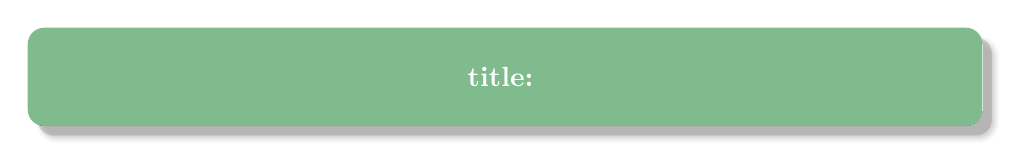
\begin{tikzpicture}
        \def\boxwidth{\linewidth}
        \def\boxheight{1.25cm}
        \def\cornerradius{6pt}
        \def\shadowshift{0.8ex}
        
        \node[fill=header,
              fill opacity=0.5,
              rounded corners=6pt,
              minimum width=\linewidth, minimum height=1.25cm,
              text=white,
              text opacity=1,
              align=center] (mainbox) at (0, 0)
        {\textbf{\usebeamerfont{title}\insertsectionhead:\;\insertsection}};

        \path (mainbox) node[rectangle, minimum width=\boxwidth, minimum height=0.989*\boxheight, rounded corners=\cornerradius, save path=\inbox] at (0, 0) {};
        \tikzset{protect=\inbox}

        \begin{scope}[transparency group, opacity=0.5]
            \fill[color=black, opacity=0.3, rounded corners=\cornerradius, blur shadow = {shadow xshift=.25ex, shadow yshift=-.25ex}] 
                (-0.5\boxwidth + \shadowshift, 0.5*\boxheight - \shadowshift) rectangle 
                (0.5\boxwidth + \shadowshift, -0.5*\boxheight - \shadowshift);
        \end{scope}
    \end{tikzpicture}
}



\newcommand\maketoc{%
    \AtBeginSection[]{%
        \icebergbackground%  <-- set the shifted background
        \begin{frame}[plain]%
            \vfill%
            \centering%
            \maketoctitleheader%
            \vfill%
        \RightSideTOC%
         
    \end{frame}
    \defaultbackground
    }
%    \AtBeginSection[]{%
%        \defaultbackground%
%        \begin{frame}[plain]%
%            \vfill%
%            \centering%
%            \maketoctitleheader%
%            \vfill%
%            \tableofcontents[currentsection, hideothersubsections]%
%            \vfill%
%      \end{frame}%
%    }%

    \AtBeginSubsection[]{%
        \icebergbackground%
        \begin{frame}[plain]%
            \vfill%
            \centering%
            \maketoctitleheader%
            \vfill%
            \tableofcontents[currentsection, currentsubsection, subsectionstyle=show/shaded/hide]%
            \vfill%
        \end{frame}%
        \defaultbackground
    }%
}%


% -------------- HEADER AND FOOTER --------------


\defbeamertemplate*{frametitle}{mytheme}{%
  \vspace{0cm}%
  {\usebeamerfont{title}\usebeamercolor[bg]{title}%
    \ifdefempty{\insertsubsectionhead}%
        {% No subsection → use section title
        \underline{\insertsectionhead:\;\insertsection}\;--\;\insertframetitle
        }%
        {% Subsection exists -> use subsection
        {\color{black}[\insertsubsectionhead]}\;\underline{\insertsectionhead:\;\insertsubsection}\;--\;\insertframetitle
        }%
    }\\[-0.55cm]%
    \hfill%
    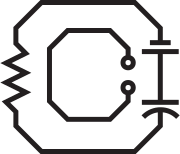
\includegraphics[height=0.635cm]{pictures/logo/c3i.pdf}%
    \hspace{0.25cm}%
    \includegraphics[height=0.635cm]{pictures/logo/m1_alpha.pdf}\par
    \vspace{-0.3cm}%
    \textcolor{UDSgreenSolidarite}{%
    \noindent\rule{\textwidth}{1pt}%
  }%
}

\defbeamertemplate*{footline}{mytheme}{%
    \leavevmode%
    \hbox{%
        \begin{beamercolorbox}%
            [wd=.33\paperwidth, ht=2.25ex, dp=1ex, center]{author in head/foot}%
            \usebeamerfont{author in head/foot}%
                \initials
        \end{beamercolorbox}%
        \begin{beamercolorbox}%
            [wd=.34\paperwidth, ht=2.25ex, dp=1ex, center]%
            {title in head/foot}%
            \usebeamerfont{title in head/foot}%
                \textbf{\inserttitle}%
        \end{beamercolorbox}%
    }%
    \begin{beamercolorbox}%
        [wd=.33\paperwidth, ht=2.25ex, dp=1ex, right]%
        {date in head/foot}%
        \hfill\usebeamerfont{date in head/foot}%
            \today{}%
        \hfill%
        \insertframenumber{} / \inserttotalframenumber%
        \hspace*{2ex}%
    \end{beamercolorbox}%
}%





% --------------- BUILD SETTINGS ----------------
\pdfcompresslevel=1
\pdfobjcompresslevel=1

% \tikzexternalize

% \dump
\csname endofdump\endcsname
\endofdump
%mylatex




% ----------------------- BEGIN DOCUMENT ------------------------

\begin{document}

\titlebackground

\begin{frame}[plain]
    \maketitle
\end{frame}

\introbackground

\begin{frame}[plain, label=intro]
    \centering
    \Large

    %\textcolor{white}{
    %    \LARGE{\textbf{\inserttitle}}\\
    %    \textbf{\textit{\insertsubtitle}}\\
    %    Par: \insertauthor\\
    %}
    \textcolor{white}{\textbf{Sujets Abordés:}}\\
    \vspace{24pt}
    \begin{tabular}{c l}
        \textcolor{UDSgreenFierte}{\faEye}
            & \textcolor{white}{Comment Visualiser les \textbf{Champs EM} sur un PCB}\\
            [0.3em]
        \textcolor{UDSgreenFierte}{\faHubspot}
            & \textcolor{white}{Comprendre l'\textbf{Effets des Materiaux} sur les champs EM}\\
            [0.3em]
        \textcolor{UDSgreenFierte}{\faLayerGroup}
            & \textcolor{white}{Comment faire un layout pour des frequences >10GHz}\\
            [0.3em]
        \textcolor{UDSgreenFierte}{\faRandom}
            & \textcolor{white}{Comment se comporte un signal jusqu'a 300GHz}\\
            [0.3em]
        \textcolor{UDSgreenFierte}{\faPastafarianism}
            & \textcolor{white}{Quantifier l'impact des \textbf{Effets Parasites}}\\
            [0.3em]
        \textcolor{UDSgreenFierte}{\faMixcloud}
            & \textcolor{white}{Comprendre la formation des \textbf{Radiations EM}}\\
            [0.3em]
        \textcolor{UDSgreenFierte}{\faMemory}
            & \textcolor{white}{Comprendre les \textbf{Sources de Signaux EM}}\\
            [0.3em]
    \end{tabular}
\end{frame}




% - TOC -
\maketoc

% ------------ SECTIONS -----------

\defaultbackground
%\input{chapters/chapter-0}
%%!TEX root = ../presentation.tex 

\section[Intro]{Introduction}
\begin{frame}{What will be covered}
    \makefigure[1.0][0.8][]{introduction/knowledge-map}
\end{frame}

\section[Intro]{Introduction}
\begin{frame}{What will be covered}
    \makefigure[1.0][0.8][]{introduction/knowledge-map}
\end{frame}


%%!TEX root = ../presentation.tex 

\section[Level 1]{Surface Ripple [20min]}
\begin{frame}{Introduction}
 Introduction des mathematiques et équation fondamentales à l'electromagnetisme
\end{frame}


\subsection[10min - Max]{EM Fields \rom{1}}
\begin{frame}{Plan}
    \begin{makelist}[\small][1.5]
        \icon{\faCheck} & Champ Vectoriel\\
        \icon[red]{\faTimes} & Divergente, Rotationnelle\\
        \icon[red]{\faTimes} & Regle de la main droite \\
        \icon[red]{\faTimes} & Equation de Maxwell
    \end{makelist}
\end{frame}

\begin{frame}{Champ Vectoriel}
\end{frame}

\begin{frame}{Divergente}

\end{frame}

\begin{frame}{Curl}
\begin{twocolumns}[0.5]
    \leftcol
        \makefigure[1.0][0.8][Cyclone Analogy]{level-1/cyclone}
    \rightcol
        \makefigure[1.0][0.6][Rotating Ball Analogy]{level-1/curl-ball}
 \end{twocolumns}
\end{frame}

\subsection[1min - Max]{Superposition \rom{1}}
\begin{frame}{Plan}
    \begin{makelist}[\small][1.5]
        \icon[red]{\faTimes} & Équation Linéaire\\
        \icon[red]{\faTimes} & Addition de Signaux
    \end{makelist}
\end{frame}

\begin{frame}{Green Theorem}
    \begin{twocolumns}[0.5]
        \leftcol
            \makefigure[1.0][0.7][Reddit moment]{level-1/green-theorem-meme}
        \rightcol
            \makefigure[1.0][0.7][Inductor Magnetic field]{level-1/inductor-magnetic-field}
    \end{twocolumns}
\end{frame}

\subsection[4min - Max]{Charge Movement}
\begin{frame}{Plan}
    \begin{makelist}[\small][1.5]
        \icon[red]{\faTimes} & Comment les Electrons bougent\\
        \icon[red]{\faTimes} & Propriété materiaux
    \end{makelist}
\end{frame}


\subsection[3min - Max]{Passive Components \rom{1}}
\begin{frame}{Plan}
    \begin{makelist}[\small][1.5]
        \icon[red]{\faTimes} & Resistance\\
        \icon[red]{\faTimes} & Condensateur \\
        \icon[red]{\faTimes} & Inducteur
    \end{makelist}
\end{frame}
%%!TEX root = ../presentation.tex

\section[Level 2]{Current Paths [30min-50min]}


\subsection[2min-Pascal]{Signal Source \rom{1}}
\begin{frame}{Plan}
    \begin{makelist}[\small][1.5]
        \icon[red]{\faTimes} & Source de tension\\
        \icon[red]{\faTimes} & Source de courant \\
    \end{makelist}
\end{frame}


\subsection[3min - Max]{Harmonics \rom{1}}
\begin{frame}{Plan}
    \begin{makelist}[\small][1.5]
        \icon[red]{\faTimes} & Transformé de fourier\\
        \icon[red]{\faTimes} & Addition de Signaux \\
        \icon[red]{\faTimes} & Taylor \\
        \icon[red]{\faTimes} & Harmonique paires/impaires
    \end{makelist}
\end{frame}

\subsection[5min-Pascal]{Propagation Speed \rom{1}}
\begin{frame}{Plan}
    \begin{makelist}[\small][1.5]
        \icon[red]{\faTimes} & Vitesse de propagation\\
        \icon[red]{\faTimes} & Speed of light\\
    \end{makelist}
\end{frame}


\subsection[5min-Pascal]{Ground planes \rom{1}}
\begin{frame}{Plan}
    \begin{makelist}[\small][1.5]
        \icon[red]{\faTimes} & Item 1\\
        \icon[red]{\faTimes} & Item 2\\
        \icon[red]{\faTimes} & GND IS NOT A SINK, IT'S A REFERENCE
    \end{makelist}
    
\end{frame}

\subsection[5min-Pascal/Max]{Induction}
\begin{frame}{Plan}
    \begin{makelist}[\small][1.5]
        \icon[red]{\faTimes} & Comment les courants sont induits \\
        \icon[red]{\faTimes} & Regle de la main droite\\
        \icon[red]{\faTimes} & Item 3
    \end{makelist}
\end{frame}

\subsection[5min-Pascal]{Current loops}
\begin{frame}{Plan}
    %Perso je splitterais cette section en 2 avec une partie plus deep dans l'iceberg
    \begin{makelist}[\small][1.5]
        \icon[red]{\faTimes} & GND Loop avec cable(Ou on place ca apres la section noise?)\\
        \icon[red]{\faTimes} & Frequency dependant loop\\
        \icon[red]{\faTimes} & Item 3
    \end{makelist}
\end{frame}

\subsection[3min-Max]{Radiation \rom{1}}
\begin{frame}{Plan}
    \begin{makelist}[\small][1.5]
        \icon[red]{\faTimes} & Simple Travelling wave\\
        \icon[red]{\faTimes} & Wavelength\\
        \icon[red]{\faTimes} & Induction is actually radiation\\
        \icon[red]{\faTimes} & Stripline radiation Pattern
    \end{makelist}
\end{frame}

\subsection[5min-Pascal]{Fil d'une année lumière de long }
% Parasitiques
\begin{frame}{Plan}
    \begin{makelist}[\small][1.5]
        \icon[red]{\faTimes} & Item 1\\
        \icon[red]{\faTimes} & Item 2\\
        \icon[red]{\faTimes} & Item 3
    \end{makelist}
\end{frame}
%%!TEX root = ../presentation.tex

\section[Level 3]{Impedance \& Reflection [20min - 1h10]}
\subsection[5min-Pascal]{Signal Source \rom{2}}
\begin{frame}{Plan}
    \begin{makelist}[\small][1.5]
        \icon[red]{\faTimes} & Type of source\\
        \icon[red]{\faTimes} & High/Low Impedance\\
        \icon[red]{\faTimes} & GPIO output circuit
    \end{makelist}
\end{frame}

\subsection[5min-Pascal]{Impédances \rom{1}}
\begin{frame}{Plan}
    \begin{makelist}[\small][1.5]
        \icon[red]{\faTimes} & PPPPP2\\
        \icon[red]{\faTimes} & Impedance dans le plan complexe\\
        \icon[red]{\faTimes} & Rappel qu'on ignore la conductance G. %On va la resortir plus tard dans la presentation
    \end{makelist}
\end{frame}


\subsection[5min-Pascal]{Réflection}
\begin{frame}{Plan}
    \begin{makelist}[\small][1.5]
        \icon[red]{\faTimes} & Bounce Diagram\\
        \icon[red]{\faTimes} & Impedance Mismatch\\
        \icon[red]{\faTimes} & Item 3
    \end{makelist}
\end{frame}
%Bounce Diagrams

\subsection[5min-Pascal]{Transmission Line \rom{1}}
\begin{frame}{Plan}
    \begin{makelist}[\small][1.5]
        \icon[red]{\faTimes} & Equation de base\\
        \icon[red]{\faTimes} & Pertes en dB (exponential decay)\\
    \end{makelist}
\end{frame}

\subsection[5min-Pascal]{Losses}
\begin{frame}{Plan}
    \begin{makelist}[\small][1.5]
        \icon[red]{\faTimes} & aaa\\
        \icon[red]{\faTimes} & Pertes en dB (exponential decay)\\
    \end{makelist}
\end{frame}
%%!TEX root = ../presentation.tex

\section[Level 4]{Noise [27min - 1h37]}
\subsection[5min-Max]{Decibel Review}
\begin{frame}{Plan}
    \begin{makelist}[\small][1.5]
        \icon[red]{\faTimes} & Pourquoi c'est important\\
        \icon[red]{\faTimes} & Analogie des dB avec le stock market\\
        \icon[red]{\faTimes} & Item 3
    \end{makelist}
\end{frame}

\begin{frame}{Signal Power}
    \centering{\underline{Signal Power in dB}}
    \begin{equation}
            P_{Signal|\unit{dB}}=10 \log{\frac{P_{\text{Signal}|\unit{W}}}{1\unit{W}}}
    \end{equation}
    \vspace{10pt}\\
    \centering{\underline{Signal Power in dBm}}
    \begin{equation}
            P_{Signal|\unit{dBm}}=10 \log{\frac{P_{\text{Signal}|\unit{mW}}}{1\unit{mW}}}
    \end{equation}
\end{frame}

\begin{frame}{System Gain}
    \centering{\underline{Voltage Gain}}
    \begin{equation}
            A_{V|\unit{dB}}=20 \log{\frac{V_{out}}{V_{in}}}
            \hspace{2.0em} \Longleftrightarrow \hspace{2.0em}
            \frac{V_{out}}{V_{in}} = 10^{\frac{A_{v}}{20}} 
    \end{equation}
    \vspace{10pt}\\
    \centering{\underline{Power Gain}}
    \begin{equation}
            A_{V|\unit{dB}}=10 \log{\frac{P_{out}}{P_{in}}}
            \hspace{2.0em} \Longleftrightarrow \hspace{2.0em}
            \frac{P_{out}}{P_{in}} = 10^{\frac{A_{P}}{10}} 
    \end{equation}
\end{frame}


\subsection[4min-Max]{Signal Source \rom{3}}
\begin{frame}{Plan}
    \begin{makelist}[\small][1.5]
        \icon[red]{\faTimes} & Random Noise Source\\
        \icon[red]{\faTimes} & Noise Power\\
        \icon[red]{\faTimes} & Source of noise in a circuit
    \end{makelist}
\end{frame}

\begin{frame}{Noise Source}
    \begin{makelist}[\small][1.5]
        \icon[red]{\faTimes} & Thermal Noise\\
        \icon[red]{\faTimes} & Environmental Noise \\
        \icon[red]{\faTimes} & Flicker Noise
    \end{makelist}
\end{frame}

\begin{frame}{Bruit Thermique - Resistance}
    \begin{twocolumns}[0.5]
        \leftcol
        Johnson-Nyquist Noise Equation:
        \begin{equation}
            V_{rms}= \sqrt{4k_BTR\Delta f}
        \end{equation}
        $k_b = 1.38\times 10^{-23}$: Boltzmann Constant [J]\\
        $T$: Temperature [K]\\
        $\Delta f$: Frequency Range\\
        $R$: Resistance [Ohm]\\
        \rightcol
        \makefigure[0.8][0.8][]{level-4/johnson-circuit}
    \end{twocolumns}
\end{frame}

\begin{frame}{Bruit Thermique - Thermique}
    %\vspace{20pt}
    \centering
    \underline{Valeurs pour 300K:}
    \begin{equation}
        V_{rms}= 0.13\cdot\sqrt{R\Delta f} \hspace{2.0em} [\SI{}{\nano\volt}]
    \end{equation}
    \makefigure[1.0][1.0]{level-4/johnson-nyquist-band}
\end{frame}

\begin{frame}{Bruit Thermique - Resistance}
    \makefigure[0.8][0.8][]{level-4/RC-noise_simpler}
\end{frame}

\begin{frame}{Bruit Thermique - Autres}
    \begin{twocolumns}[0.5]
        \leftcol
        \centering
        \underline{Bruit Condensateur:}
        \begin{equation}
            V_{rms}= \sqrt{\frac{k_BT}{C}}
        \end{equation}
        \rightcol
        \centering
        \underline{Bruit Inducteur:}
        \begin{equation}
            \overline{I_{n}}= \sqrt{\frac{k_BT}{L}}
        \end{equation}
    \end{twocolumns}
\end{frame}

\begin{frame}{Bruit Thermique - Applications}
    \maketable{thermal-noise}
\end{frame}

%Radio Noise
%https://www.itu.int/rec/R-REC-P.372/en
\begin{frame}{Bruits Environnementaux}
    \begin{makelist}[\small][1.5]
        \icon{\faBolt} & \textbf{Atmospheriques:} Éclairs, Effets Corona, etc...\\
        \icon{\faHouzz} & \textbf{Industriel:} Lignes HV, Lampes Fluorescentes, etc...\\
        \icon{\faSun} & \textbf{Solaire:} Vents solaires\\
        \icon{\faMeteor} & \textbf{Cosmique:} Effets colectif des étoiles (8MHz-1.5GHz), CMB, Quasar, Pulsar, Chaos Gods\\
        \icon{\faFrown} & \textbf{Psychologique:} Toi qui fait pas tes lectures\\
    \end{makelist}
\end{frame}

\subsection[2min-Max]{Noise Spectrum}
\begin{frame}{Plan}
    \begin{makelist}[\small][1.5]
        \icon[red]{\faTimes} & Frequency dependant noise power\\
        \icon[red]{\faTimes} & Demo avec type de bruit (red, white, brown, etc..)
    \end{makelist}
\end{frame}

\begin{frame}{Average Power of a Signal}
    \begin{equation}
        P_{n}=\lim_{T \rightarrow \infty}\frac{1}{T}\int_{0}^{T}n^{2}(t) \,dt
   \end{equation}
    \vspace{10pt}\\
    \begin{equation}
        \int_{0}^{\infty}S_{x}(f) \, df = \lim_{T \rightarrow \infty}\frac{1}{T}\int_{0}^{T}x^{2}(t) \, dt
   \end{equation}
\end{frame}

\subsection[3min-Max]{Harmonics \rom{2}}
\begin{frame}{Plan}
    \begin{makelist}[\small][1.5]
        \icon[red]{\faTimes} & Gauss representation in frequency domain of a sine wave\\
        \icon[red]{\faTimes} & Sinc function\\
        \icon[red]{\faTimes} & Item 3
    \end{makelist}
\end{frame}
%
%Sinc function

\subsection[5min-Max]{Signal to Noise Ratio (SNR)}
\begin{frame}{Plan}
    \begin{makelist}[\small][1.5]
        \icon[red]{\faTimes} & Why it matters\\
        \icon[red]{\faTimes} & How can you tell the SNR you need\\
        \icon[red]{\faTimes} & Shannon-Hartley Theorem\\
        \icon[red]{\faTimes} & Application: DAC,ADC\\
        \icon[red]{\faTimes} & Application: Example for Voyager 1 Detection \href{https://www.seti.org/detecting-voyager-1-ata}{Link}
    \end{makelist}
\end{frame}

\begin{frame}{Definition}
    \begin{equation}
        SNR = \frac{P_{\text{Signal}|\unit{W}}}{P_{\text{Noise}|\unit{W}}}=P_{\text{Signal}|\unit{dB}} - P_{\text{Noise}|\unit{dB}}
    \end{equation}
\end{frame}

\begin{frame}{Shannon-Hartley}
    \begin{equation}
        C = BW \cdot \log_{2}\left( 1+\frac{P_{\text{Signal}|\unit{W}}}{P_{\text{Noise}|\unit{W}}} \right)
    \end{equation}
    \begin{makelist}[\small][1.5]
        \icon[blue]{\faCloudversify} & C: Canal Capacity [Bit/s]\\
        \icon[blue]{\faChartArea} & BW: Canal Bandwidth [Hz]
    \end{makelist}
\end{frame}
% 
% 
\begin{frame}{Determining SNR}
    Mettre tableau avec resolution et SNR
\end{frame}

\subsection[5min-Pascal]{Jitter}
\begin{frame}{Plan}
    \begin{makelist}[\small][1.5]
        \icon[red]{\faTimes} & Item 1\\
        \icon[red]{\faTimes} & Item 2\\
        \icon[red]{\faTimes} & Item 3
    \end{makelist}
\end{frame}


\subsection[5min-Pascal]{Eye diagram \rom{1}}
\begin{frame}{Plan}
    \begin{makelist}[\small][1.5]
        \icon[red]{\faTimes} & Item 1\\
        \icon[red]{\faTimes} & Item 2\\
        \icon[red]{\faTimes} & Item 3
    \end{makelist}
\end{frame}


\pauseframe%

%%!TEX root = ../presentation.tex 

\section{Level 7: Field lines and Fringes}

\subsection{E-field}
\subsection{B-field}
\subsection{Skew, loss}
\subsection{Skin effect}
\subsection{EMI}

%%!TEX root = ../presentation.tex 


\section{Dielectric Depths}
\subsection{Conduction}
\subsection{Loss tangent}
\subsection{Frequency-dependant resistances}
\subsection{Current Bunching}
\subsection{Stackup}
% Comment lire une datasheet diélectrique
% Comment optimiser un stackup
% Avantages / désavantages de certains matériaux

%%!TEX root = ../presentation.tex 

\section[Level 7]{Field lines and Fringes [20min-2h27]}

\subsection[5min-Pascal]{Ground Planes \rom{2}}
\begin{frame}{Plan}
    \begin{makelist}[\small][1.5]
        \icon[red]{\faTimes} & Ground Bounce\\
        \icon[red]{\faTimes} & Vias pour changer de layers\\
        \icon[red]{\faTimes} & item 3
    \end{makelist}
\end{frame}

\subsection[5min-Pascal]{Waveguide \rom{2}}
\begin{frame}{Plan}
    \begin{makelist}[\small][1.5]
        \icon[red]{\faTimes} & stripline Field\\
        \icon[red]{\faTimes} & Microstrip Field\\
        \icon[red]{\faTimes} & CPWG, GCPWG field\\
        \icon[red]{\faTimes} & Vias
    \end{makelist}
\end{frame}

\begin{frame}{When it's a waveguide}    
    \maketable{model-threshold}
\end{frame}

%Transmission line 3?

\subsection[10min-Max-Pascal]{Matériaux \rom{3}}
\begin{frame}{Plan}
    \begin{makelist}[\small][1.5]
        \icon[red]{\faTimes} & Susceptibility\\
        \icon[red]{\faTimes} & Polarization and Magnetisation\\
        \icon[red]{\faTimes} & Effective Complex Permittivity\\
        \icon[red]{\faTimes} & Frequency dependance\\
    \end{makelist}
\end{frame}

\begin{frame}{Rappel}
    \begin{twocolumns}[0.4]
        \leftcol
            Electric Permittivity [F/m]:
            \begin{equation*}
                \varepsilon =\varepsilon_r \varepsilon_0
            \end{equation*}
            Refractive Index:
            \begin{equation*}
                n =\frac{\sqrt{\varepsilon \mu}}{\sqrt{\varepsilon_0 \mu_0}} = \sqrt{\varepsilon_r \mu_r}
            \end{equation*}
            Permittivitée Complexe:
            \begin{equation*}
                \varepsilon = \epsilon_1 + j \epsilon_2 = (n+jk)^2
            \end{equation*}
        \rightcol
            Dans les sections précédentes, nous avons vu pourquoi les propriété des matériaux sont définies avec \textbf{nombres complexe} $\mathbb{C}$.
    \end{twocolumns}
\end{frame}

\begin{frame}{Rappel}
    \centering
    \begin{twocolumns}[0.4]
        \leftcol
            \centering
            \underline{Intensitée du Champ Électrique}
            \begin{equation*}
                \efield \rightarrow [\SI{}{\volt\per\meter}]
            \end{equation*}
            \underline{Densitée de Flux Électrique}
            \begin{equation*}
                \eflux \rightarrow [\SI{}{\coulomb\per\meter\squared}]
            \end{equation*}
            \underline{Relation}
            \begin{equation*}
                \eflux = \varepsilon \efield
            \end{equation*}
        \rightcol
            \centering
            \underline{Intensitée de Champ Magnétique}
            \begin{equation*}
                \mfield \rightarrow [\SI{}{\ampere\per\meter}]
            \end{equation*}
            \underline{Densitée de Flux Magnétique}
            \begin{equation*}
                \mflux \rightarrow [\SI{}{\weber\per\meter\squared} \;\; ou \;\; \SI{}{\tesla}]
            \end{equation*}
            \underline{Relation}
            \begin{equation*}
                \mflux = \mu \mfield
            \end{equation*}
    \end{twocolumns}
\end{frame}


\begin{frame}{Susceptibility}
    La susceptibilitée est une autre valeur pour définir les propriétés de matériaux.
    \begin{equation}
        \begin{aligned}
            \suse &=  \varepsilon_r - 1 \hspace{2em} \text{Electric Susceptibility}\\
            \susm &=  \mu_r - 1 \hspace{2em} \text{Magnetic Susceptibility}
        \end{aligned}
    \end{equation}
    \vspace{20pt}
    Vacuum Susceptibility is always 0
\end{frame}

\begin{frame}{Polarization Density}
    \begin{twocolumns}[0.6]
        \leftcol
        La densitée de polarisation représente la \textbf{contribution des dipôles électriques} du matériau qui \textbf{s'alignent} en réponse à un champs $\efield$
        \begin{equation*}
            \eflux = \varepsilon \efield \hspace{1em} \rightarrow \hspace{1em} \eflux = \varepsilon_0 \efield + \pola
        \end{equation*}
        \vspace{10pt}
        \begin{equation*}
            \begin{aligned}
                \pola &=  \left(\varepsilon - \varepsilon_0 \right) \efield\\
                &= \varepsilon_0 \suse \efield
            \end{aligned}
        \end{equation*}
        \rightcol
    \makefigure[1.0][0.6][]{level-7/polarization}
    \end{twocolumns}
    \centering
    $\pola$ représente également l'énergie électrique que le matériau accumule.
\end{frame}

\begin{frame}{Effective Complex Permittivity}
    \begin{twocolumns}[0.5]
     \leftcol
         Conversion to phasor form:
        \begin{equation*}
            \begin{aligned}
                \nabv \times \mfield &= \ddt{\eflux} + \ecurrent \\
                &= j\omega \eflux + \sigma \efield\\
                &= j\omega \varepsilon \efield + \sigma \efield\\
            \end{aligned}
        \end{equation*}
            Developpement:
        \begin{equation*}
            \begin{aligned}
                j\omega \varepsilon \efield + \sigma \efield &= j\omega \left(\epsilon_1 - j \epsilon_2\right)\efield + \sigma \efield \\
                &= j\omega \epsilon_1 \efield +  \left( \sigma + \omega \epsilon_2 \right)\efield \\
                &= j\omega \left(\epsilon_1 - j \epsilon_2 - j \frac{\sigma}{\omega}\right)\efield\\
            \end{aligned}
        \end{equation*}
    \rightcol
        \begin{equation*}
            \begin{aligned}
                \omega \varepsilon_1 &: \text{Ability to store electric energy}\\
                \omega \varepsilon_2 &: \text{Dielectric damping loss}\\
                \sigma &: \text{Conductivity loss}
            \end{aligned}
        \end{equation*}
    \end{twocolumns}
\end{frame}

\begin{frame}{Effective Complex Permittivity}
    \centering
    \underline{Effective Complex Relative Permittivity}
    \begin{equation}
        \varepsilon_e = \left(\epsilon_1 - j\epsilon_2 - j\frac{\sigma}{\omega}\right)\frac{1}{\varepsilon_0}
    \end{equation}
    This term describe the properties of \textbf{non-homogeneous} materials. It can be seen as an average of all the individual relative permittivities.

\end{frame}

\subsection[5min-Pascal]{EM Fields \rom{2}}
\begin{frame}{Plan}
    \begin{makelist}[\small][1.5]
        \icon[red]{\faTimes} & Skin effect\\
        \icon[red]{\faTimes} & EMI\\
        \icon[red]{\faTimes} & Item 3
    \end{makelist}
\end{frame}

\begin{frame}{Skin Depth of Different Materials}
    %\begin{center}
    %    \textbf{1oz PCB = $\SI{35}{\micro\meter}$}
    %\end{center}

    \maketable{skin-depth}
\end{frame}



%%!TEX root = ../presentation.tex 

\section[Bonus Level 11]{S-Parameters and Smith Charts [17min-3h35]}
\subsection[5min-Pascal/Max]{S-Parameters}
\begin{frame}{Plan}
    \begin{makelist}[\small][1.5]
        \icon[red]{\faTimes} & Item 1\\
        \icon[red]{\faTimes} & Item 2\\
        \icon[red]{\faTimes} & Item 3
    \end{makelist}
\end{frame}

\subsection[5min-Pascal/Max]{Smith Charts}
\begin{frame}{Plan}
    \begin{makelist}[\small][1.5]
        \icon[red]{\faTimes} & Item 1\\
        \icon[red]{\faTimes} & Item 2\\
        \icon[red]{\faTimes} & Item 3
    \end{makelist}
\end{frame}

\subsection[5min-Pascal]{Impedance Matching Network}
\begin{frame}{Plan}
    \begin{makelist}[\small][1.5]
        \icon[red]{\faTimes} & Item 1\\
        \icon[red]{\faTimes} & Item 2\\
        \icon[red]{\faTimes} & Item 3
    \end{makelist}
\end{frame}

\subsection[2min-Max]{Standing Waves}
\begin{frame}{Plan}
    \begin{makelist}[\small][1.5]
        \icon[red]{\faTimes} & Item 1\\
        \icon[red]{\faTimes} & Item 2\\
        \icon[red]{\faTimes} & Item 3
    \end{makelist}
\end{frame}


%\subsection{Fin premiere Partie}
\chapterframe

%%!TEX root = ../presentation.tex 

\section[Bonus Level 12]{Non-linearity Valley [14min-3h49]}
\subsection[5min-Pascal]{Passive Component \rom{3}}
\begin{frame}{Plan}
    \begin{makelist}[\small][1.5]
        \icon[red]{\faTimes} & Nonlinear passive component models\\
        \icon[red]{\faTimes} & 
    \end{makelist}
\end{frame}

\subsection[3min-Max]{Superposition \rom{3}}
\begin{frame}{Plan}
    \begin{makelist}[\small][1.5]
        \icon[red]{\faTimes} & Superposition breaks\\
        \icon[red]{\faTimes} & Item 2\\
        \icon[red]{\faTimes} & Item 3
    \end{makelist}
\end{frame}


\subsection[5min-Max]{Harmonics \rom{3}}
\begin{frame}{Plan}
    \begin{makelist}[\small][1.5]
        \icon[red]{\faTimes} & How non-linearity create harmonics\\
        \icon[red]{\faTimes} & Item 2\\
        \icon[red]{\faTimes} & Item 3
    \end{makelist}
\end{frame}

\subsection[3min-Max]{Intermodulation}
\begin{frame}{Plan}
    \begin{makelist}[\small][1.5]
        \icon[red]{\faTimes} & Item 1\\
        \icon[red]{\faTimes} & Item 2\\
        \icon[red]{\faTimes} & Item 3
    \end{makelist}
\end{frame}

\subsection[3min-Max]{Crossmodulation}
\begin{frame}{Plan}
    \begin{makelist}[\small][1.5]
        \icon[red]{\faTimes} & Item 1\\
        \icon[red]{\faTimes} & Item 2\\
        \icon[red]{\faTimes} & Item 3
    \end{makelist}
\end{frame}
% À réévaluer

%%!TEX root = ../presentation.tex 

\section{Bonus Level 13: Infrared Chasm [10min  - 3h59]}
\subsection{When the equations fails [5min - Max]}
\subsection{Electron vibration frequency [2min - Max]}
\subsection{Blackbody Radiation [3min - Max]}


%%!TEX root = ../presentation.tex 

\section{Final Boss: Integrated Photonics [18min - 4h17]}
\subsection{RF Blocks can also be used to guide light [5min - Max]}
\subsection{We can make circuits with light [3min - Max]}
\subsection{We can manipulate light using Electrical Signals [5min - Max]}
\subsection{We can use photonics to generate and manipulate Microwave Signals [5min - Max]}

%\input{chapters/chapter-12}
%%!TEX root = ../presentation.tex 

\section[Bonus Level 13]{Infrared Chasm [10min-3h59]}

\subsection[5min-Max]{Impedance \rom{4}}
\begin{frame}{Plan}
    \begin{makelist}[\small][1.5]
        \icon[red]{\faTimes} & When the equations fails\\
    \end{makelist}
\end{frame}

\subsection[5min-Max]{Matériaux \rom{7}}
\begin{frame}{Plan}
    \begin{makelist}[\small][1.5]
        \icon[red]{\faTimes} & Electron Vibration Frequency\\
        \icon[red]{\faTimes} & Black-Body Radiation\\
    \end{makelist}
\end{frame}

\subsection[5min-Max]{Plasmonics}
\begin{frame}{Plan}
    \begin{makelist}[\small][1.5]
        \icon[red]{\faTimes} & item 1\\
        \icon[red]{\faTimes} & item 2\\
    \end{makelist}
\end{frame}



%%!TEX root = ../presentation.tex 

\section[Final Boss]{Integrated Photonics [18min-4h17]}
\subsection[5min - Max]{RF Blocks can also be used to guide light}
\begin{frame}{Plan}
    \begin{makelist}[\small][1.5]
        \icon[red]{\faTimes} & Item 1\\
        \icon[red]{\faTimes} & Item 2\\
        \icon[red]{\faTimes} & Item 3
    \end{makelist}
\end{frame}

\subsection[3min - Max]{We can make circuits with light}
\begin{frame}{Plan}
    \begin{makelist}[\small][1.5]
        \icon[red]{\faTimes} & Item 1\\
        \icon[red]{\faTimes} & Item 2\\
        \icon[red]{\faTimes} & Item 3
    \end{makelist}
\end{frame}

\subsection[5min - Max]{We can manipulate light using Electrical Signals}
\begin{frame}{Plan}
    \begin{makelist}[\small][1.5]
        \icon[red]{\faTimes} & Item 1\\
        \icon[red]{\faTimes} & Item 2\\
        \icon[red]{\faTimes} & Item 3
    \end{makelist}
\end{frame}

\subsection[5min - Max]{We can use photonics to generate and manipulate Microwave Signals}
\begin{frame}{Plan}
    \begin{makelist}[\small][1.5]
        \icon[red]{\faTimes} & Item 1\\
        \icon[red]{\faTimes} & Item 2\\
        \icon[red]{\faTimes} & Item 3
    \end{makelist}
\end{frame}




%!TEX root = ../presentation.tex
\pascalbackground

\begin{frame}{Comment fonctionne un crystal}
    \begin{twocolumns}[0.66]
        \leftcol
            \begin{itemize}
                \item Oscillateur utilisant l'effet piézoélectrique
                \item Déformation mécanique d'une matrice cristalline
                \item Génère un champ électrique
                \item Effet inverse possible!
                \bigskip
                \item Fréquence de résonance
                \item Q factor beaucoup plus élevé que circuit RLC équivalent
            \end{itemize}
        \makefigure[1][0.35]{level-5/piezoelectric-effect}
        \rightcol
            \begin{maketikzfigure}[1][0.66]
                \draw (0, 6) node[vcc] {};
                \draw (0, 6) to [short] (-1, 6) to 
                [R, l=$R_1$] (-1, 4) to
                [american inductor, l=$L_1$] (-1, 2) to
                [C, l=$C_1$] (-1, 0) to
                [short] (0, 0) 
                node[ground] {};

                \draw (0, 6) to [short] (1, 6) to
                [C, l=$C_2$] (1, 0) to 
                [short] (0, 0);
            \end{maketikzfigure}
    \end{twocolumns}
\end{frame}

\begin{frame}{Comment résonne un crystal}
    \begin{twocolumns}[0.33]
        \leftcol
            \begin{maketikzfigure}
                \draw (0, 6) node[vcc] {};
                \draw (0, 6) to [short] (-1, 6) to 
                [R, l=$R_1$, color=UDSviolet] (-1, 4) to
                [american inductor, l=$L_1$, color=orange] (-1, 2) to
                [C, l=$C_1$, color=blue] (-1, 0) to
                [short] (0, 0) 
                node[ground] {};

                \draw (0, 6) to [short] (1, 6) to
                [C, l=$C_2$, color=red] (1, 0) to 
                [short] (0, 0);
            \end{maketikzfigure}
        \rightcol

            \begin{maketikzfigure}
            \begin{axis}[
              width=12cm, height=6.5cm,
              axis lines=left,
              xlabel={$f$}, ylabel={$Z$},
              xmin=0, xmax=1, ymin=0, ymax=1,
              xtick=\empty, ytick=\empty,
              clip=false
            ]

            \addplot[ultra thick, accent, smooth]
              coordinates {
                (0.02, 0.92) (0.10, 0.60) (0.22, 0.22)             % falling, capacitive
                (0.30, 0.30) (0.38, 0.55) (0.46, 0.80)             % rising to parallel resonance
                (0.52, 0.88) (0.62, 0.62) (0.78, 0.48) (0.98,0.36) % roll-off
              };

            \def\xFs{0.26}
            \def\xFr{0.50}

            \draw[dashed] (axis cs:\xFs,0) -- (axis cs:\xFs, 1);
            \draw[dashed] (axis cs:\xFr,0) -- (axis cs:\xFr, 1);

            \draw[color=UDSviolet, thick] (axis cs:0, 0.20) -- (axis cs:1, 0.20);

            \node[above] at (axis cs:\xFs, 1) {$f_s$};
            \node[above] at (axis cs:\xFr, 1) {$f_r$};

            \node[anchor=south west] at (axis cs:0.02, 1) {\small Capacitif};
            \node[anchor=south]      at (axis cs:0.38, 1) {\small Inductif};
            \node[anchor=south east] at (axis cs:0.98, 1) {\small Capacitif};

            \node[below] at (axis cs:\xFs,0) {\scriptsize Résonance Série};
            \node[below] at (axis cs:\xFr,-0.1) {\scriptsize Résonance Parallèle};

            \end{axis}
                
            \end{maketikzfigure}
    \end{twocolumns}
\end{frame}

\begin{frame}{Crystal sur un microcontrôleur}
    \ctikzset{bipoles/capacitor/height=0.5}
    \ctikzset{bipoles/capacitor/width=0.2}
    \ctikzset{logic ports/scale=0.5}
    \begin{maketikzfigure}

        \draw (4, 0) node [dipchip,
            num pins = 8,
            hide numbers,
            external pins width=0.3,
            external pad fraction=4,
            ](IC){};

            \node [right, font=\tiny] at (IC.bpin 1) {OSC2};
            \node [right, font=\tiny] at (IC.bpin 4) {OSC1};


            \draw[thick] (IC.pin 1) to [short] ($(IC.pin 1) - (1.5, 0)$) to
            [piezoelectric, color=accent] ($(IC.pin 4) - (1.5, 0)$) to
            [short] (IC.pin 4);

            \only<1, 3>{
                \draw[thick] ($(IC.pin 1) - (1.5, 0)$) to
                [C, l=$C_1$] ($(IC.pin 1) - (3.5, 0)$);
                \draw[thick] ($(IC.pin 4) - (1.5, 0)$) to
                [C, l=$C_2$] ($(IC.pin 4) - (3.5, 0)$);
            }
            \only<2, 4->{
                \draw[thick] ($(IC.pin 1) - (1.5, 0)$) to
                [C, l=$C_1$, color=accent2] ($(IC.pin 1) - (3.5, 0)$);
                \draw[thick] ($(IC.pin 4) - (1.5, 0)$) to
                [C, l=$C_2$, color=accent2] ($(IC.pin 4) - (3.5, 0)$);
            } 

            \draw[thick] ($(IC.pin 1) - (3.5, 0)$) to [short] ($(IC.pin 4) - (3.5, 0)$)
            to [short]   ($(IC.pin 4) - (3.5, 1)$) node[ground]{};


            \only<3->{
                \draw[dashed] (IC.bpin 1) to [short] ($(IC.pin 1) + (1.5, 0)$) to [open]
                ($(IC.pin 4) + (1.5, 0)$) to [short] (IC.bpin 4);

                \draw ($(IC.pin 1) + (1.5, 0)$) to [inline not, color=accent2] ($(IC.pin 4) + (1.5, 0)$);
            }

            \only<4->{
                \draw[->, color = accent]    ($(IC.pin 1) + (2, 0)$)    -- ($(IC.pin 4) + (2, 0)$)    node[midway, below, sloped] {$+\ang{180}$};
                \draw[<-, color = UDSviolet] ($(IC.pin 1) - (0.75, 0)$) -- ($(IC.pin 4) - (0.75, 0)$) node[midway, below, sloped] {$+\ang{180}$};
            }
    \end{maketikzfigure}
\end{frame}

\begin{frame}{Condensateur de charge}
    \begin{twocolumns}
        \leftcol
        \only<1>{
        \begin{itemize}
            \item Les circuits de lecture CMOS d'oscillateur rajoutent une phase de $\ang{180}$
            \item Phase doit être compensée pour atteindre $\ang{360}$
            \item Condensateurs viennent compléter le modèle RLCC du crystal
            \item Crystaux calibrés pour des valeurs de condensateurs $C_L$
        \end{itemize}
        }

        \only<2->{
            \begin{tabular}{l | c}
                \multicolumn{2}{c}{\textbf{\textbf{ESC-16-20S-4X}}}\\
                \hline
                \textbf{Frequency}             & $\SI{16}{\mega\hertz}$\\
                \textbf{Frequency Tolerance}   & $\pm 30\,ppm$\\
                \textbf{Frequency Stability}   & $\pm 50\,ppm$\\
                \textbf{Shunt Capacitance}     & $\SI{7}{\pico\farad}$\\
                \textbf{Load Capacitance}      & $\SI{20}{\pico\farad}$\\
                \textbf{Operating Temperature} & $\SI{-10}{\celsius} à \SI{70}{\celsius}$\\
                \textbf{Storage Temperature}   & $\SI{-55}{\celsius} à \SI{125}{\celsius}$\\
                \textbf{ESR Max}               & $\SI{40}{\ohm}$\\
            \end{tabular}
        }

        \rightcol
        \only<2>{
            \makefigure[1][0.25]{level-5/hc49}
        }
        \begin{align*}
            C_1 &= C_2 = 2 \cdot (C_L - C_{stray})\\
            C_L &= \dfrac{C_1 \cdot C_2}{C_1 + C_2} + C_{stray}\\
            \vspace{18pt}
            C_{stray} \sim \SI{5}{\pico\farad}\\
        \end{align*}
        \only<3->{
            \begin{align*}
                C_1 &= C_2 = 2 \cdot (\SI{20}{\pico\farad} - \SI{10}{\pico\farad})\\
                C_1 &= C_2 = \SI{20}{\pico\farad}\\
            \end{align*}
        }
    \end{twocolumns}
\end{frame}

\begin{frame}{Types d'oscillateurs}
    \begin{tabular}{c | c | c | c}
        \textbf{XO} & \textbf{VCXO} & \textbf{TCXO} & \textbf{OCXO}\\
        \hline
        \textit{Crystal Oscillator} & 
        \textit{\textbf{V}oltage-\textbf{C}ontrolled} &
        \textit{\textbf{T}emperature-\textbf{C}ontrolled} &
        \textit{\textbf{O}ven-\textbf{C}ontrolled}\\
    \end{tabular}
\end{frame}


% - END -

\titlebackground
\thankyouframe


% VOTE
\introbackground
\begin{frame}
    \centering
    \Large

    \textcolor{white}{\LARGE{\textbf{Prochain PPPPP}}}\\
    \vspace{18pt}

    \textcolor{white}{
    \LARGE{\textbf{Bonnes pratiques de design}}}\\
    \vspace{24pt}

    \begin{itemize}
        \item \textcolor{white}{Comment choisir ses composantes et optimiser son BOM?}
        \item \textcolor{white}{Comment bien conçevoir un symbole et un footprint?}
        \item \textcolor{white}{Bonnes pratiques de schémas}
        \item \textcolor{white}{Bonnes pratiques de layout}
        \item \textcolor{white}{Communication avec fabricants, assembleurs et programmeurs}
    \end{itemize}
\end{frame}

\defaultbackground
\begin{frame}[allowframebreaks]{Références}
    \printbibliography
\end{frame}



\end{document}
